\documentclass[whitelogo]{template/tudelft-report}
\usepackage[utf8]{inputenc}
\usepackage{changes}
\usepackage{graphicx}
\usepackage{adjustbox}
\usepackage{listings}

%bibliography imports


\begin{document}
%% Use Roman numerals for the page numbers of the title pages and table of
%% contents.
\frontmatter

%% Uncomment following 19 lines for a cover with a picture on the lower half only
%\title[tudelft-white]{Title}
%\subtitle[tudelft-cyan]{Optional subtitle}
%\author[tudelft-white]{J.\ Random Author}
%\affiliation{Technische Universiteit Delft}
%\coverimage{cover.jpg}
%\titleoffsetx{10cm}
%\titleoffsety{10cm}
%\afiloffsetx{1cm}
%\afiloffsety{18cm}
%\covertext[tudelft-white]{
%    \textbf{Cover Text} \\
%    possibly \\
%    spanning 
%    multiple 
%    lines
%    \vfill
%    ISBN 000-00-0000-000-0
%}
%\makecover

%% Uncomment following 16 lines for a cover with a picture on the lower half only
\title[tudelft-white]{Hall Effect}
\subtitle[tudelft-black]{Onderzoeken 5}
\author[tudelft-white]{Brian de Keijzer \\ Julia Norbart}
\affiliation{De Haagse Hogeschool}
\covertext[tudelft-white]{ % Dit moet makkelijker/mooier kunnen
    Vak \qquad\quad Onderzoeken 5 \\
    Klas\qquad\quad NH2B \\
    Docent \quad\space\space dr. ir. J. B. Oostinga \\
    \vfill
    \today
}
\setpagecolor{tudelft-cyan}
\makecover[split]



%% Include an optional title page.
\begin{titlepage}


\begin{center}

%% Insert the TU Delft logo at the bottom of the page.

%% Print the title in cyan.
{\makeatletter
\largetitlestyle\fontsize{64}{94}\selectfont\@title
%\largetitlestyle\color{tudelft-cyan}\Huge\@title
\makeatother}

%% Print the optional subtitle in black.
{\makeatletter
\ifx\@subtitle\undefined\else
    \bigskip
   {\tudsffamily\fontsize{22}{32}\selectfont\@subtitle}    
    %\titlefont\titleshape\LARGE\@subtitle
\fi
\makeatother}

\bigskip
\bigskip

by
%door

\bigskip
\bigskip

%% Print the name of the author.
{\makeatletter
%\largetitlefont\Large\bfseries\@author
\largetitlestyle\fontsize{26}{26}\selectfont\@author
\makeatother}

\bigskip
\bigskip

\vfill

\begin{tabular}{lll}
    Names: & Brian de Keijzer & Julia Norbart \\
    Studentnumbers: & 16011015 & 16083946 \\
    Emails: & 16011015@student.hhs.nl & 16083946@student.hhs.nl
\end{tabular}
%% Only include the following lines if confidentiality is applicable.

%\centering{
\includegraphics{cover/logo_black}}


\end{center}

\begin{tikzpicture}[remember picture, overlay]
    \node at (current page.south)[anchor=south,inner sep=0pt]{
        
\includegraphics{cover/logo_black}
    };
\end{tikzpicture}

\end{titlepage}



\chapter*{Abstract}
\setheader{Abstract}

Abstract\ldots

\begin{flushright}
{\makeatletter\itshape
    \@author \\
    Delft, \today
\makeatother}
\end{flushright}

Samenvatting: de samenvatting bevat een korte beschrijving van wat er gemeten/onderzocht is. Daarnaast worden de belangrijkste resultaten en conclusies opgenomen. Het stukje tekst (ca. een half A4-tje) moet uitnodigend zijn om het verslag te gaan lezen; dit bepaalt veelal of het verslag gelezen wordt of niet.



\tableofcontents

%% Use Arabic numerals for the page numbers of the chapters.
\mainmatter

%% Import chapters
\chapter{Introduction}

Hoofdstuk 1 Inleiding: het doel van de inleiding is de lezer nieuwsgierig en duidelijk te maken wat de lezer kan verwachten. De inleiding bevat de context, de achtergrond, de probleemstelling en/of onderzoeksvragen.


This document is intended to be both an example of the TU Delft \LaTeX{} template for reports and theses, as well as a short introduction to its use. It is not intended to be a general introduction to \LaTeX{} itself,\footnote{We recommend \url{http://en.wikibooks.org/wiki/LaTeX} as a reference and a starting point for new users.} and we will assume the reader to be familiar with the basics of creating and compiling documents.

Instructions on how to use this template under Windows and Linux, and which \LaTeX{} packages are required, can be found in \texttt{README.txt}.

\section{Document Structure}

Since a report, and especially a thesis, might be a substantial document, it is convenient to break it up into smaller pieces. In this template we therefore give every chapter its own file. The chapters (and appendices) are gathered together in \texttt{report.tex}, which is the master file describing the overall structure of the document. \texttt{report.tex} starts with the line
\begin{quote}
    \texttt{\textbackslash documentclass\{tudelft-report\}}
\end{quote}
which loads the TU Delft report template. The template is based on the \LaTeX{} \texttt{book} document class and stored in \texttt{tudelft-report.cls}. The document class accepts several comma-separated options. The default language is English, but this can be changed to Dutch (\emph{e.g.}, for bachelor theses) by specifying the \texttt{dutch} option:
\begin{quote}
    \texttt{\textbackslash documentclass[dutch]\{tudelft-report\}}
\end{quote}
Furthermore, hyperlinks are shown in blue, which is convenient when reader the report on a computer, but can be expensive when printing. They can be turned black with the \texttt{print} option. This will also turn the headers black instead of cyan.

If the document becomes large, it is easy to miss warnings about the layout in the \LaTeX{} output. In order to locate problem areas, add the \texttt{draft} option to the \texttt{\textbackslash documentclass} line. This will display a vertical bar in the margins next to the paragraphs that require attention. Finally, the \texttt{nativefonts} option can be used to override the automatic font selection (see below).

This template has the option to automatically generate a cover page with the \texttt{\textbackslash makecover} command. See the next section for a detailed description.

The contents of the report are included between the \texttt{\textbackslash begin\{document\}} and \texttt{\textbackslash end\{document\}} commands, and split into three parts by
\begin{enumerate}
\item\texttt{\textbackslash frontmatter}, which uses Roman numerals for the page numbers and is used for the title page and the table of contents;
\item\texttt{\textbackslash mainmatter}, which uses Arabic numerals for the page numbers and is the style for the chapters;
\item\texttt{\textbackslash appendix}, which uses letters for the chapter numbers, starting with `A'.
\end{enumerate}
The title page is defined in a separate file, \emph{e.g.}, \texttt{title.tex}, and included verbatim with \texttt{\textbackslash input\{title\}}.\footnote{Note that it is not necessary to specify the file extension.} Additionally, it is possible to include a preface, containing, for example, the acknowledgements. An example can be found in \texttt{preface.tex}. The table of contents is generated automatically with the \texttt{\textbackslash tableofcontents} command. Chapters are included after \texttt{\textbackslash mainmatter} and appendices after \texttt{\textbackslash appendix}. For example, \texttt{\textbackslash input\{chapter-1\}} includes \texttt{chapter-1.tex}, which contains this introduction.

The bibliography, finally, is generated automatically with
\begin{quote}
    \texttt{\textbackslash bibliography\{report\}}
\end{quote}
from \texttt{report.bib}. The bibliography style is specified in \texttt{tudelft-report.bst}, which is a modified version of \texttt{apsrev4-1.bst} (from REVTeX) designed to also display the titles of referenced articles. The template will automatically generate clickable hyperlinks if a URL or DOI (digital object identifier) is present for the reference. As an example, we cite the paper by Nobel laureate Andrei Geim and his pet hamster \citep{Geim2001}. Although it is possible to manage the bibliography by hand, we recommend using EndNote (available from Blackboard) or JabRef (available from \url{http://jabref.sourceforge.net/}).

\section{Cover and Title Page}

This template will automatically generate a cover page if you issue the \texttt{\textbackslash makecover} command. There are two formats for the cover page: one with a page-filling (`bleeding')
illustration, with the title(s) and author(s) in large ultrathin typeface, and the other where the illustration fills the lower half of the A4, whereas title(s), author(s) and additional
text are set in the standard sans-serif font on a plain background with a color chosen by the user. The last option is selected by the optional key \texttt{split}: \texttt{\textbackslash makecover[split]} yields
a page with the illustration on the lower half. All illustrations are bleeding, in accordance with the TU Delft style.

Before generating the cover, you need to provide the information to put on it. This can be done with the following commands:
\begin{itemize}
\item\texttt{\textbackslash title[Optional Color]\{Title\}} \\
    This command is used to provide the title of the document. The title
    title is also printed on the spine. If you use a title page (see below), this information will be used there as well.
    As the title, subtitle and author name are printed directly over the cover photo, it will often be necessary to adjust the print color in order to have
    sufficient contrast between the text and the background. The optional color argument is used for this.
\item\texttt{\textbackslash title[Optional Color]\{Subtitle\}} \\
    This command is used to provide a subtitle for the document. If you use a title page (see below), this information will be used there as well.
    It possible to adjust the print color in order to have
    sufficient contrast between the text and the background -- the optional color argument is used for this.
\item\texttt{\textbackslash author\{J.\ Random Author\}} \\
    This command specifies the author. The default color is \texttt{tudelft-white}, but this may be adjusted in the same way as the titles.
\item\texttt{\textbackslash affiliation\{Technische Universiteit Delft\}} \\
    The affiliation is the text printed vertically on the front cover. It can be the affiliation, such as the university or department name, or be used for the document type (\emph{e.g.}, Master's thesis). The default color is again \texttt{tudelft-white}, adjustable through the \texttt{color} option.
\item\texttt{\textbackslash coverimage\{cover.jpg\}} \\
    With this command you can specify the filename of the cover image. The image is stretched to fill the full width of the front cover (including the spine if a back cover is present).
\item\texttt{\textbackslash covertext\{Cover Text\}} \\
    If a back cover is present, the cover text is printed on the back. Internally, this text box is created using the \LaTeX{} \texttt{minipage} environment, so it supports line breaks.
\item\texttt{\textbackslash titleoffsetx\{OffsetX\},\textbackslash titleoffsety\{OffsetY\}}
    If the cover page contains a page-filling picture (i.e., \texttt{split} is not specified with the \texttt{makecover} command, the best position of the title depends a lot on the picture chosen for it. The lower left corner of the minipage containing title, subtitle and author is 
    specified by these two commands. The offsets are measured from the top left corner of the page. 
\item\texttt{\textbackslash afiloffsetx\{AfilX\}, \textbackslash afiloffsety\{AfilY\}}
    specifies the lower left corner of the text containing the affiliation, measured from the top left corner of the page. 
\end{itemize}

In addition to \texttt{[split]}, the \texttt{\textbackslash makecover} command accepts several additional options for customizing the layout of the cover. 
The most important of these is \texttt{back}. Supplying this option will generate a back cover as well as a front, including the spine. Since this requires a page size slightly larger than twice A4 (to make room for the spine), and \LaTeX{} does not support different page sizes within the same document, it is wise to create a separate file for the cover. \texttt{cover.tex} contains an example. The recommended page size for the full cover can be set with
\begin{quote}
    \textbackslash geometry\{papersize=\{1226bp,851bp\}\}
\end{quote}
after the document class and before \texttt{\textbackslash begin\{document\}}.

The other options \texttt{\textbackslash makecover} accepts are
\begin{itemize}
\item\texttt{nospine} \\
    If a back cover is generated, the title will also be printed in a black box on the spine. However, for smaller documents the spine might not be wide enough. Specifying this option disables printing the title on the spine.
\item\texttt{frontbottom} \\
    By default the black box on the front is situated above the blue box. Specifying this option will place the black box below the blue one.
\item\texttt{spinewidth} \\
    If a back cover is present, this option can be used to set the width of the spine. The default is \texttt{spinewidth=1cm}.
\item\texttt{frontboxwidth}, \texttt{frontboxheight}, \texttt{backboxwidth}, \texttt{backboxheight} \\
    As their names suggest, these options are used to set the width and height of the front (black) and back (blue) boxes. The default widths and heights are \texttt{4.375in} and \texttt{2.1875in}, respectively.
\item\texttt{x}, \texttt{y} \\
    The blue and black boxes touch each other in a corner. The location of this corner can be set with these options. It is defined with respect to the top left corner of the front cover. The default values are \texttt{x=0.8125in} and \texttt{y=3in}.
\item\texttt{margin} \\
    This option sets the margin between the borders of the boxes and their text. The default value is \texttt{12pt}.
\end{itemize}

For a thesis it is desirable to have a title page within the document, containing information like the thesis committee members. To give you greater flexibility over the layout of this page, it is not generated by a command like \texttt{\textbackslash makecover}, but instead described in the file \texttt{title.tex}. Modify this file according to your needs. The example text is in English, but Dutch translations are provided in the comments. Note that for a thesis, the title page is subject to requirements which differ by faculty. Make sure to check these requirements before printing.

\section{Chapters}

Each chapter has its own file. For example, the \LaTeX{} source of this chapter can be found in \texttt{chapter-1.tex}. A chapter starts with the command
\begin{quote}
    \texttt{\textbackslash chapter\{Chapter title\}}
\end{quote}
This starts a new page, prints the chapter number and title and adds a link in the table of contents. If the title is very long, it may be desirable to use a shorter version in the page headers and the table of contents. This can be achieved by specifying the short title in brackets:
\begin{quote}
    \texttt{\textbackslash chapter[Short title]\{Very long title with many words which could not possibly fit on one line\}}
\end{quote}
Unnumbered chapters, such as the preface, can be created with \texttt{\textbackslash chapter*\{Chapter title\}}. Such a chapter will not show up in the table of contents or in the page header. To create a table of contents entry anyway, add
\begin{quote}
    \texttt{\textbackslash addcontentsline\{toc\}\{chapter\}\{Chapter title\}}
\end{quote}
after the \texttt{\textbackslash chapter} command. To print the chapter title in the page header, add
\begin{quote}
    \texttt{\textbackslash setheader\{Chapter title\}}
\end{quote}

Chapters are subdivided into sections, subsections, subsubsections, and, optionally, paragraphs and subparagraphs. All can have a title, but only sections and subsections are numbered. As with chapters, the numbering can be turned off by using \texttt{\textbackslash section*\{\ldots\}} instead of \texttt{\textbackslash section\{\ldots\}}, and similarly for the subsection.
\section{\textbackslash section\{\ldots\}}
\subsection{\textbackslash subsection\{\ldots\}}
\subsubsection{\textbackslash subsubsection\{\ldots\}}
\paragraph{\textbackslash paragraph\{\ldots\}}
Lorem ipsum dolor sit amet, consectetur adipisicing elit, sed do eiusmod tempor incididunt ut labore et dolore magna aliqua. Ut enim ad minim veniam, quis nostrud exercitation ullamco laboris nisi ut aliquip ex ea commodo consequat. Duis aute irure dolor in reprehenderit in voluptate velit esse cillum dolore eu fugiat nulla pariatur. Excepteur sint occaecat cupidatat non proident, sunt in culpa qui officia deserunt mollit anim id est laborum.

\section{Fonts and Colors}

The fonts used by this template depend on which version of \LaTeX{} you use. Regular \LaTeX, \emph{i.e.}, if you compile your document with with \texttt{latex}, \texttt{pslatex} or \texttt{pdflatex}, will use Utopia for text, Fourier for math and Latin Modern for sans-serif and monospaced text. 
However, if you want to adhere to the TU Delft house style, you will need to use \XeLaTeX, as it supports TrueType and OpenType fonts. Compiling with \texttt{xelatex} will use Arial for most titles and text, Courier New for monospace and Cambria for math. If you want to haf a sans-serif font for the
main text, while using \texttt{latex}, \texttt{pslatex} or \texttt{pdflatex}, you can use the option \texttt{noroman} in the report style: \texttt{\textbackslash usepackage[\ldots,noroman]{tudelft-report}}. For document and part titles,  TU Delft Ultra Light is used. For quotes, columns and text in boxes, you use Georgia. If you want to use \XeLaTeX, but do not want to use the TU Delft house style fonts, you can add the \texttt{nativefonts} option to the document class. This will still use  TU Delft Utra Light and Arial on the cover, but not for the body of the document. If you need to use these fonts for certain sections in the main text, they are available via \texttt{\textbackslash tudrmfamily} (Georgia) and \texttt{\textbackslash tudtitlefamily} (TU Delft Utra Light).

\begin{quote}
  You have to learn the rules of the game. And then you have to play better than anyone else.\\
  \emph{Albert Einstein}
\end{quote}

The corporate colors of the TU Delft are cyan, black and white, available via \texttt{\textbackslash color\{{\color{tudelft-cyan}tudelft-cyan}\}}, \texttt{\textbackslash color\{{\color{tudelft-black}tudelft-black}\}} (which differs slightly from the default \texttt{\textbackslash color\{black\}}) and \texttt{\textbackslash color\{tudelft-white\}}, respectively. Apart from these three, the house style defines the basic colors \texttt{\color{tudelft-sea-green}tudelft-sea-green}, \texttt{\color{tudelft-green}tudelft-green}, \texttt{\color{tudelft-dark-blue}tudelft-dark-blue}, \texttt{\color{tudelft-purple}tudelft-purple}, \texttt{\color{tudelft-turquoise}tudelft-turquoise} and \texttt{\color{tudelft-sky-blue}tudelft-sky-blue}, as well as the accent colors \texttt{\color{tudelft-lavendel}tudelft-lavendel}, \texttt{\color{tudelft-orange}tudelft-orange}, \texttt{\color{tudelft-warm-purple}tudelft-warm-purple}, \texttt{\color{tudelft-fuchsia}tudelft-fuchsia}, \texttt{\color{tudelft-bright-green}tudelft-bright-green} and \texttt{\color{tudelft-yellow}tudelft-yellow}.


\chapter{Theory}
In this chapter the fundamental physics behind the Hall effect will be discussed. The Hall coefficient and charge carrier density will also be discussed. These both are unique material properties, which are related to each other. How so will become clear at the end of this chapter.

\section{The Hall effect}
When an electric current $I$ flows through a conductor perpendicular to a magnetic field $B$, it results in a transverse force $F_m$ on the moving charge carriers due to the magnetic field. Those charge carriers are pushed to one side of the conductor due to the Hall effect. All the chargers are building up at one side of the conductor. Because of this, there is a measurable voltage difference between the two sides of the conductor. This measurable voltage difference is called the Hall voltage. This Hall voltage is due is a potential difference due to the Hall effect. This effect is called after E.H. Hall, who discovered the Hall effect in 1897 [bron?]. The change in the direction of the current $I$ is caused by the magnetic force. This force is given by [bron?]:
    \begin{equation}
        \vec F = q\cdot (\vec E + \vec v \times \vec B)
        \label{eq:force}
    \end{equation}
%   
    \begin{table}[!htbp]
    \centering
    \caption{The quantities belonging to Equation \ref{eq:force}.}
    \label{table:force}
    \begin{tabular}{|c|c|c|}
    \hline
    \textbf{Quantity}   & \textbf{Description}           & \textbf{Unit}            \\ \hline
    $q$                  & Electrical charge    & {[}C{]}                     \\ \hline
    $\vec E$                  & Electric field strength         & {[}V/m{]}                     \\ \hline
    $\vec v$                  & Drift speed           & {[}m/s{]}                     \\ \hline
    $\vec B$                  & Magnetic field & {[}T{]} \\ \hline
    \end{tabular}
    \end{table}
    \begin{figure}[!htbp]
    \begin{center}
        \begin{minipage}[t]{0.45\textwidth}
            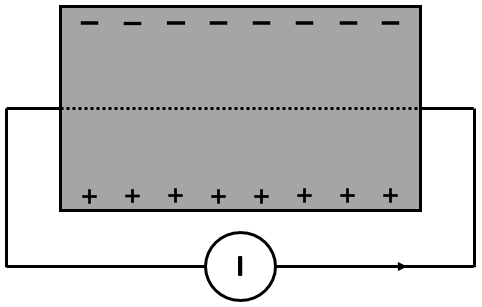
\includegraphics[scale=0.45]{figuren/theorie_e_rechtdoor.png}
            \caption{A schematic of the coil configuration.} \label{fig:schematic_setup_magnets}
        \end{minipage}
        \begin{minipage}[t]{0.45\textwidth}
            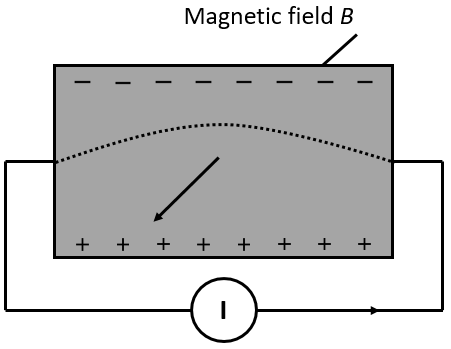
\includegraphics[scale=0.47]{figuren/theorie_e_afbuigen.png}
             \caption{The schematic setup for the experimental setup of the Hall effect.}\label{fig:schematic_hall_effect}
        \end{minipage}
    \end{center}
    \end{figure}
\begin{figure} [!htbp]
    \centering
    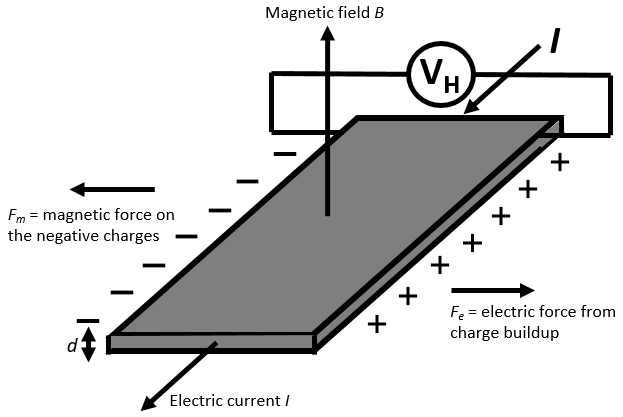
\includegraphics[scale=0.7]{figuren/schematic_forces.png}
    \caption{A schematic representation of the force on a current due to the Hall effect.}
    \label{fig:schematic_force}
\end{figure}
The quantities belonging to Equation \ref{eq:force} are defined in Table \ref{table:force}.
Because of this force, the positive and negative charges will have an acceleration in the direction of the force. This results in a change of the path of the charges. Which will lead to a potential difference.\\
Without magnetic field and thus without the force, the charges will go straight from one side of the material to the other, see Figure \ref{fig:schematic_setup_magnets}. When there is a magnetic field, the path changes in a curve, see Figure \ref{fig:schematic_hall_effect}. The potential different due to this effect is called the Hall Voltage. The Hall voltage is given by:
    \begin{equation}
        U_H = v_d\cdot B \cdot d
        \label{eq:Hall voltage}
    \end{equation}
With the distance $d$ between the positive and negative side of the plate. 
There also is current of the electrical charge in the negative direction with respect to the electon current, this is the conventional 'hole' current. This current can be written as:
    \begin{equation}
        I_x = n\cdot tw\cdot (-v_d)\cdot (-e)
        \label{eq:Hole current}
    \end{equation}
The quantities belonging to Equation \ref{eq:Hole current} are defined in Table \ref{table:Hole current}.
    \begin{table}[!htbp]
    \centering
    \caption{The quantities belonging to Equation \ref{eq:Hole current}.}
    \label{table:Hole current}
    \begin{tabular}{|c|c|c|}
    \hline
    \textbf{Quantity}   & \textbf{Description}           & \textbf{Unit}            \\ \hline
    $n$                  & Charge carrier density    & {[}Electrons/m^3{]}                     \\ \hline
    $tw$                  & The cross-sectional area         & {[}m^2{]}                     \\ \hline
    $-v_d$                  & Drift speed           & {[}m/s{]}                     \\ \hline
    $-e$                  & Charge of each electron & {[}C{]} \\ \hline
    \end{tabular}
    \end{table}
In which $e$ is the elementary charge, being equal to \cite{elementarycharge}:
\begin{equation}
    e = (1.602... \cdot 10^{-19} \pm 6.1 \cdot 10^{-9}) \quad \text{[C]} \label{eq:e}
\end{equation}
This equation can be solved for \emph{w} and plugged into Equation \ref{eq:Hall voltage} resulting in the Hall voltage:
 \begin{equation}
        U_H = \frac{1}{n \cdot e} \frac{B \cdot I}{d}. \label{eq:Hall Voltage2}
    \end{equation}

\section{Hall coefficient \& charge carrier density}
The Hall effect can be used to determine the Hall coefficient, which is an unique material property. this can be done by writing equation \ref{eq:Hall Voltage2} in the form of
    \begin{equation}
        U_H = R_H \frac{B I}{d} \label{eq:hallspanning_with_coefficient}
    \end{equation}
Where $R_H=\frac{1}{n \cdot e}$ is called the Hall coefficient. For silver $R_H$ is equal to \cite{apparatus_silver}:
    \begin{equation}
        \mid R_H \mid = (8,9 \pm 2) \cdot 10^{-11}  \quad \text{[m$^3$C$^{-1}$]} \label{eq:hallcoefficient_lit}
    \end{equation}
When the electric charge of the charge carriers in a material is known, Equation \ref{eq:hallspanning_with_coefficient} can be used to determine the charge carrier density. The charge carrier density $n$ is the number of charge carriers per volume.  The charge carrier density denotes the number of charge carriers per volume. It is measured in m$^{-3}$. As any density it can depend on position. It should not be confused with the charge density, which is the number of charges per volume at a given energy [bron?]. The charge carrier density is received by rewriting Equation \ref{eq:Hall Voltage2} to:
    \begin{equation}
        n = \frac{1}{e} \cdot \frac{1}{R_H}
    \end{equation}
In which $R_H$ is the Hall coefficient and $e$ the elementary charge. The charge carrier density cannot be directly measured. Therefor it has to be experimentally determined. This can be done by using the Hall effect. Silver for example has a charge carrier density of \cite{apparatus_silver}:
    \begin{equation}
        n = (6.6 \pm 2)\cdot 10^{28} \quad \text{[m$^{-3}$]} \label{eq:ccdensity_lit}
    \end{equation}
It is important to note that the uncertainties of Equation \ref{eq:hallcoefficient_lit} and Equation \ref{eq:ccdensity_lit} are not given by their source. However, their experimental results in comparison with the literature value are given. The difference between these two have been chosen as the uncertainties for Equation \ref{eq:hallcoefficient_lit} and Equation \ref{eq:ccdensity_lit}.
\chapter{Experimental procedure}
This chapter consists of the experimental setup and measurement procedure. Firstly the required apparatus is specified. After the apparatus is known, the calibration of the magnetic field is explained. At last the measurement procedure for the Hall voltage is discussed.

\section{Experimental setup}
The experimental setup can be divided into two sections. The first section is used to create a magnetic field. A schematic of this part of the experimental setup is shown in Figure \ref{fig:schematic_setup_magnets}. The maximum continues current supported by the coils is 5 A, this current is supplied by the power supply unit (PSU). It is possible to supply the coils with a higher current, for example 15 A. However, this has to be in a relatively short time frame. This is so the coils do not get damaged. A list of the required apparatus is shown in Figure \ref{fig:apparatus}, which can be found in Appendix-A. The power supply used to power the coils has to be able to deliver a current up to 5 A. This current is measured with a TTi 1604 digital multimeter. This multimeter is used for all current and voltage measurements. The necessary magnetic field strength to be created is between 0.1 and 0.6 T \cite{apparatus_silver}.\\
    \begin{figure}[!htbp]
    \begin{center}
        \begin{minipage}[t]{0.45\textwidth}
            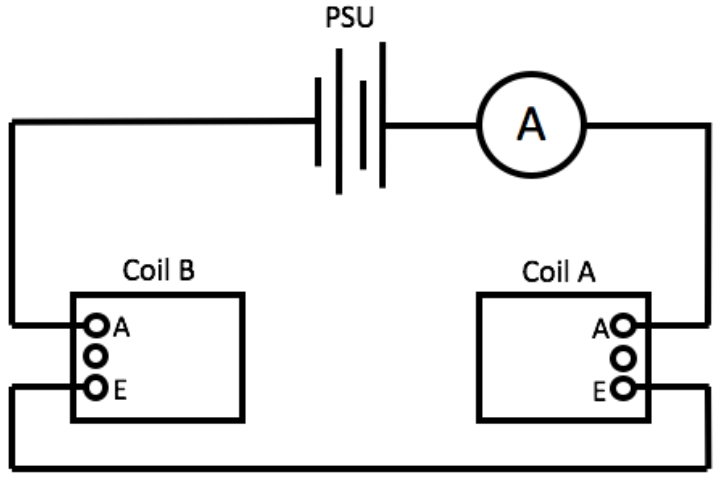
\includegraphics[scale=0.35]{figuren/schematic_setup_magnets.png}
            \caption{A schematic of the coil configuration.} \label{fig:schematic_setup_magnets}
        \end{minipage}
        \begin{minipage}[t]{0.45\textwidth}
            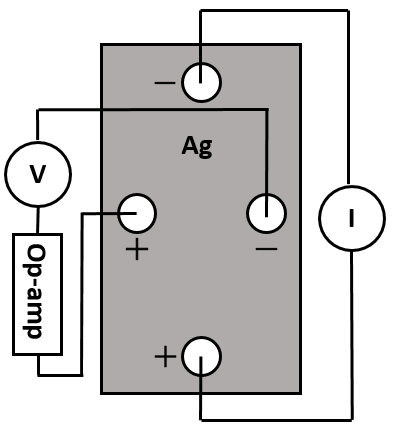
\includegraphics[scale=0.5]{figuren/schematic_hall_voltage.png}
             \caption{The schematic setup for the experimental setup of the Hall effect.}\label{fig:schematic_hall_effect}
        \end{minipage}
    \end{center}
    \end{figure}
The second section of the experimental setup consists of the material on which the Hall voltage is measured. A schematic of this part of the experimental setup can be seen in Figure \ref{fig:schematic_hall_effect}. The PSU which supplies the current through the material must be able to supply up to 20 A. The Hall voltage is measured by a multimeter. An operational amplifier (Op-amp) might be needed to amplify the Hall voltage. The need for an Op-amp depends on the material used. Silver for example, has a Hall voltage of 5 $\mu$V when a current of 15 A flows through the material, in a 0,2 T magnetic field perpendicular to the flow of current \cite{halleffectzilver}. 5 $\mu$V cannot be measured by the TTi 1604 multimeter, therefor an Op-amp circuit is required to amplify the voltage to an order of magnitude which can be measured by the TTi 1604 \cite{dmm}. The chosen Op-amp is an AD521, which can amplify the signal up to one thousand times. With a maximum output voltage of 30 V \cite{AD521}. Note that the exact amplification of the Op-amp has to be determined before it is used in a measurement. This can be done by using two multimeters and a signal generator to apply a known signal and measure the Op-amps output. At last a computer with CASSY Lab is required for the data-acquisition of the Combi B-Sensor S. The Combi B-Sensor S measures the strength of the magnetic field at the Hall apparatus center with respect to earth's magnetic field.
    
\section{Magnetic field calibration}
The magnetic field strength created by the coils as a function of the current through them has to be known. This is due to the fact the magnetic field strength sensor does not fit in between the coils while the Hall apparatus is present. By experimenting it can be seen that the magnetic field in between the coils is homogeneous. For this reason a model for the magnetic field as function of current through the coils can respectively simply be made. This part of the experimental setup can be seen in Figure \ref{fig:cal_setup}.\\
    \begin{figure}[!htbp]
    \begin{center}
        \begin{minipage}[t]{0.45\textwidth}
            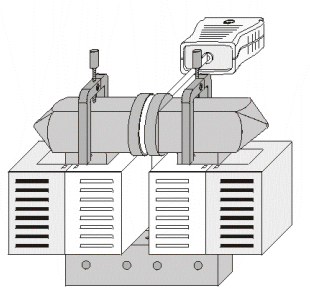
\includegraphics[scale=0.8]{figuren/schematic_calibration.png}
            \caption{Calibration of the magnetic field \\ schematically  \cite{halleffectzilver}.}\label{fig:cal_setup}
        \end{minipage}
        \begin{minipage}[t]{0.45\textwidth}
            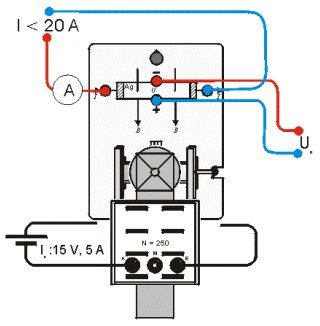
\includegraphics[scale=0.8]{figuren/experimental_setup.png}
            \caption{The wiring diagram for the experimental setup of the Hall effect \cite{halleffectzilver}.}\label{fig:experimental_setup}
        \end{minipage}
    \end{center}
\end{figure}
The magnetic field as a function of the amount of current through the coils is calibrated as follows. The current through the coils is increased by steps of 0,1 A from 0 to 5 A. At each step the strength of the magnetic field is measured. This data can be used to create a mathematical model, which later on can be used to calculate the magnetic field strength when the current through the coils is known. This is done in Chapter 4.1. It is important to emphasize that the hysteresis characteristics of the soft metal surrounded by the coils is ignored due to simplicity.

\section{Hall voltage measurement}
The experimental setup should look like Figure \ref{fig:experimental_setup} when the coils and Hall apparatus are setup according to respectively Figure \ref{fig:schematic_setup_magnets} and Figure \ref{fig:schematic_hall_effect}. A Hall voltage can be create by two physical situations. When the current flow in the material is constant, the strength of the magnetic field perpendicular to this current flow has to increase. Or when the strength of the magnetic field is constant, the current has to increase. Either one will create a Hall voltage, as long as Equation \ref{eq:Hall Voltage2} is not equal to zero. Which means that $B$ and $I$ have to be larger then 0. \\
In case of the current through the coils being a constant, the magnetic field strength perpendicular to the material has to be increased. This is done by starting with 0 A through the coils, going up all the way to 5 A in steps of 0,5 A. This way the magnetic field $B$ can be calculated because the current through the coils is known, the Hall voltage at this specific magnetic field strength can also be measured. This should result in a linear model, since Equation \ref{eq:Hall Voltage2} is linear. \\
The same thing goes for a constant magnetic field strength of for example 0,2 T. The current through the material is varied from 0 to 20 A in steps of 1 A. This should also result in a linear model because of the reason stated above. \\
In this experiment a Hall apparatus with silver has been used in a 0,3 T magnetic field. It it important to note that two different silver apparatuses have been used with part number '58681 B2' \& '58681'. Why this is important will become clear in Chapter 6. When measuring the hall voltage, the offset voltage has to be determined first. This is done by turning off the magnetic field and measuring the offset voltage across the Hall apparatus. Once this is done the magnetic field can be turned on, which will result in a voltage increase due to the Hall effect. The actual difference between the measured voltage with magnetic field and the offset voltage is the voltage due to the Hall effect. One can also reverse the magnetic field to remove any longitudinal impurities in the force vector on the charge carriers.

\section{Python simulation}
Equation \ref{eq:Hall Voltage2} can be used to simulate experimental results. These simulations can be used to verify the actual experimental results while measuring.
    \begin{equation}
        U_H = \frac{1}{n \cdot e} \frac{B \cdot I}{d} \tag{\ref{eq:Hall Voltage2}}
    \end{equation}
Multiple physical situations have been modelled. In each situation all variables except for one, have been kept constant. These situations give insight in how the Hall voltage changes for different materials in different situations. In each situation Equation \ref{eq:e} has been used as the value for the elementary charge $e$.
\chapter{Measurements (Voorkeur naar eigen informatieve titel)}

Hoofdstuk 4 Resultaten: in dit hoofdstuk wordt de presentatie van de data gegeven in de vorm van grafieken en/of korte functionele tabellen. Leg uit wat je gemeten hebt, waar de data staat (in dit hoofdstuk / paragraaf of bijlage). Leg de grafieken uit en geef vooral aan wat de lezer uit de grafiek kan afleiden. Maak ook een voorbeeldberekening (inclusief de gebruikte formules) n.a.v. de data met direct daarna de onzekerheidsberekening. Bij een eenvoudige berekening (vb. wet van Ohm) hoeft geen voorbeeld berekening opgenomen te worden. De rest kan in een tabel of in een extra kolom bij de datatabel. Zijn er voor de grafieken al berekeningen nodig dan komen de berekeningen direct na de data presentatie. Bespreek de trendlijnen, pas regressieanalyse toe en breng de koppeling met de theorie aan. Schijf eerst tekst voordat je een tabel of grafiek presenteert.

Bij meetresultaten alleen relevante tabellen en/of grafieken (zie ook bijlagen) zodat de leesbaarheid niet verstoord wordt. Bij voorkeur een grafiek in plaats van een tabel. Een grafiek laat in één oogopslag het verloop van de relatie tussen de grootheden zien. De tabel moet wel in het verslag opgenomen worden; dit kan in de tekst (kleine tabel) of in een bijlage.

\section{Uncertainty Calculations}

\section{Data Analytics}
\chapter{Conclusion}
The research question as given in Chapter 1 is:
 \begin{itemize}
     \item  What is the charge carrier density of silver?
 \end{itemize}
The Hall coefficient of silver is determined to be:
    \begin{equation}
        R_H = (8.3 \pm 2) \cdot 10^{-11} \quad \text{[m$^3$C$^{-1}$]}
    \end{equation}
The literature value for the Hall coefficient of silver is \cite{apparatus_silver}:
    \begin{equation}
        \mid R_{H}_{ literature} \mid = (8,9 \pm 2) \cdot 10^{-11}  \quad \text{[m$^3$C$^{-1}$]}
    \end{equation}
The charge carrier density of silver is determined to be:
    \begin{equation}
        n = (7.4 \pm 2)\cdot 10^{28} \quad \text{[m$^{-3}$]}.
    \end{equation}
Of which the literature value is equal to \cite{apparatus_silver}:
    \begin{equation}
        n_{literature} = (6.6 \pm 2)\cdot 10^{28} \quad \text{[m$^{-3}$]}
    \end{equation}
It can be concluded that the measured Hall coefficient and charge carrier density of silver are in agreement with the literature values. The physical results for silver are also similar to the simulation results as presented in Chapter 4.5. Therefor it can be conclude that the used model is correct for silver. Moreover, there is no reason to believe that this model (Equation \ref{eq:Hall Voltage2}) is incorrect for other materials in different physical situations.
\chapter{Discussion}

Discussie: wanneer de discussie te lang voor de conclusie wordt dan kan na de conclusie een apart item Discussie opgenomen worden. In de discussie wordt de onderbouwing van je interpretatie van de resultaten opgenomen met daaruit voortvloeiend mogelijke aanbevelingen. Aanbevelingen kunnen zijn: verbetering meetopstelling, andere meetmethode, aanvullend onderzoek verrichten e.d.


\nocite{*}
\bibliographystyle{IEEEtran}
\bibliography{references}

%% Use letters for the chapter numbers of the appendices.
\appendix

\newpage

\chapter{Figures}

    \begin{figure}[!htbp]
    \begin{center}
    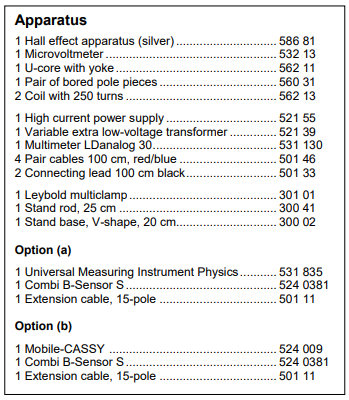
\includegraphics[scale=0.9]{figuren/apparatus.png}
    \end{center}
    \caption{A screenshot of the required apparatus \cite{halleffectzilver}.}\label{fig:apparatus}
    \end{figure}

    \begin{figure}[!htbp]
    \begin{center}
    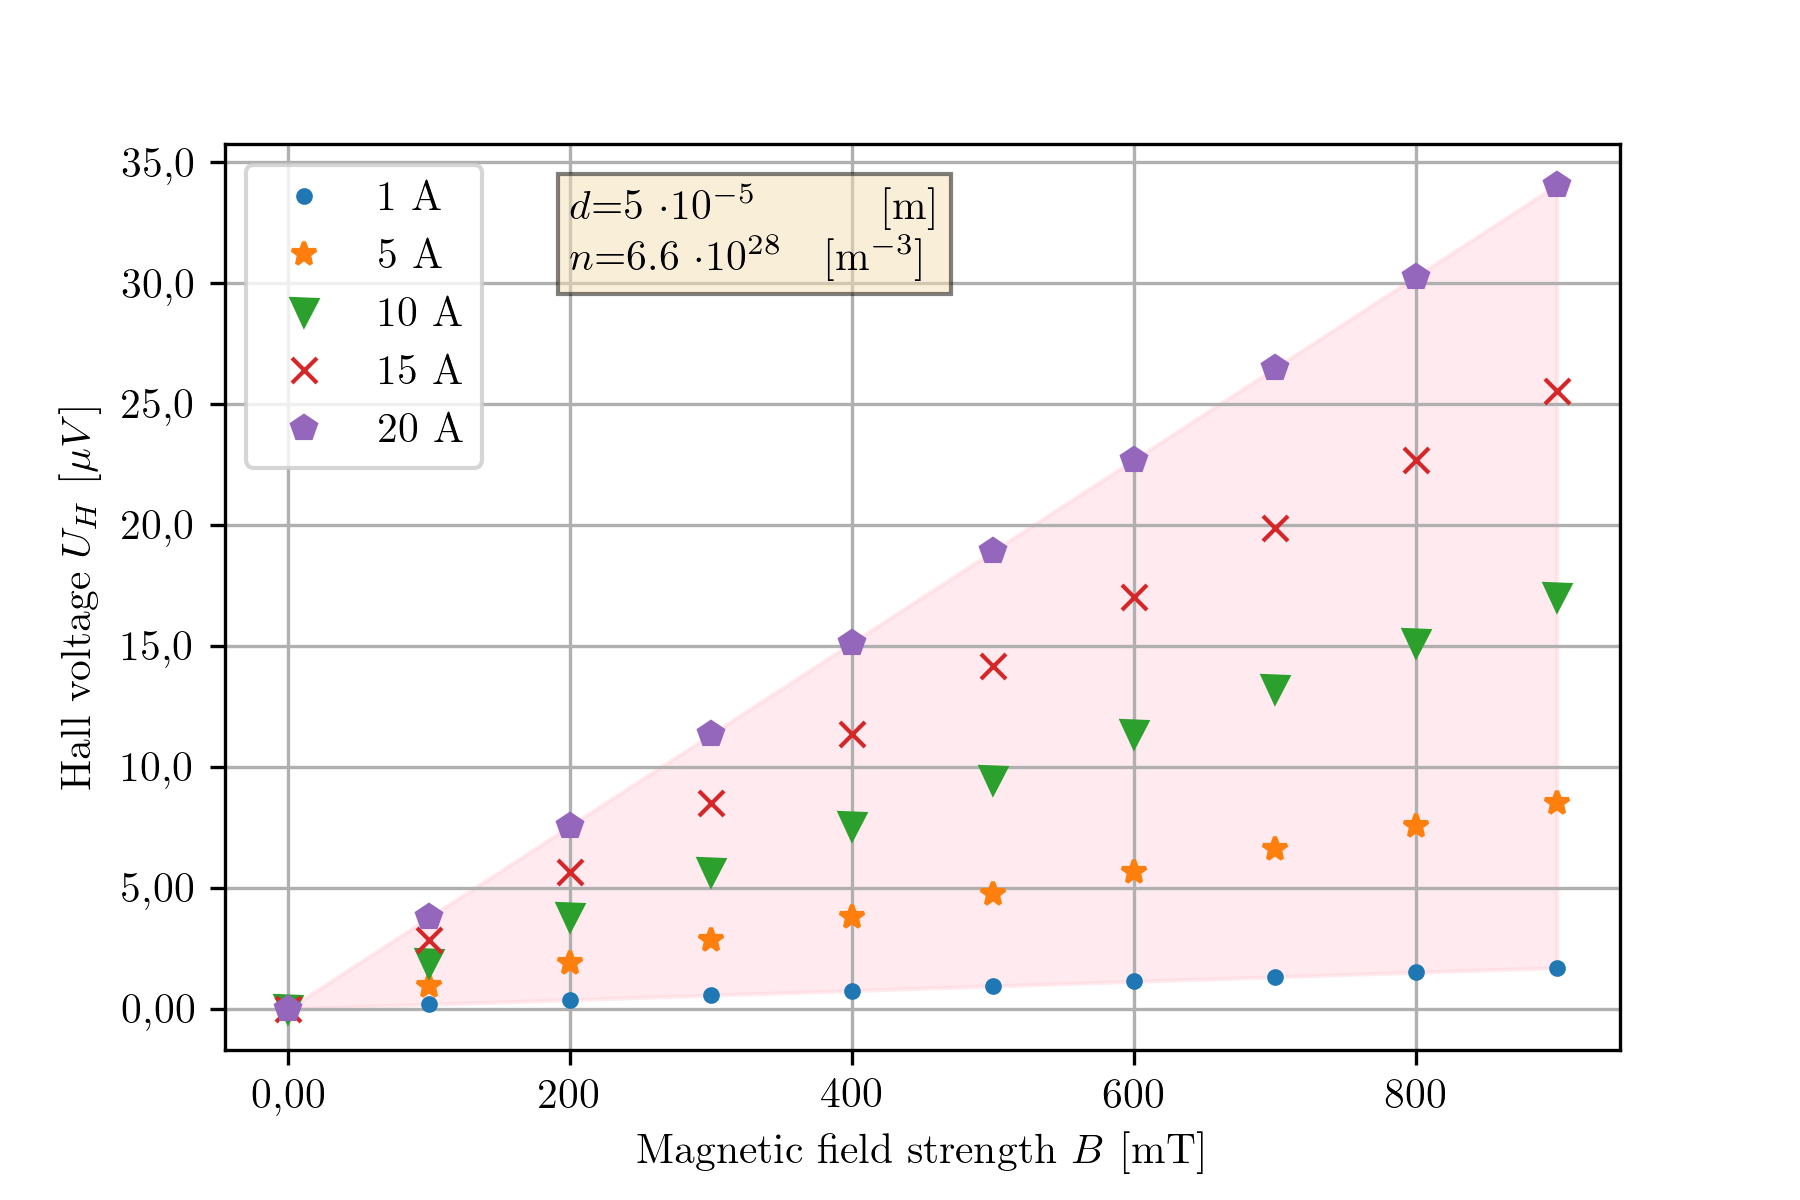
\includegraphics[scale=0.9]{figuren/simulatie/B.png}
    \end{center}
    \caption{Simulation result of Formula \ref{eq:Hall Voltage2}.}  \label{fig:sim_B}
    \end{figure}
    
    \begin{figure}[!htbp]
    \begin{center}
    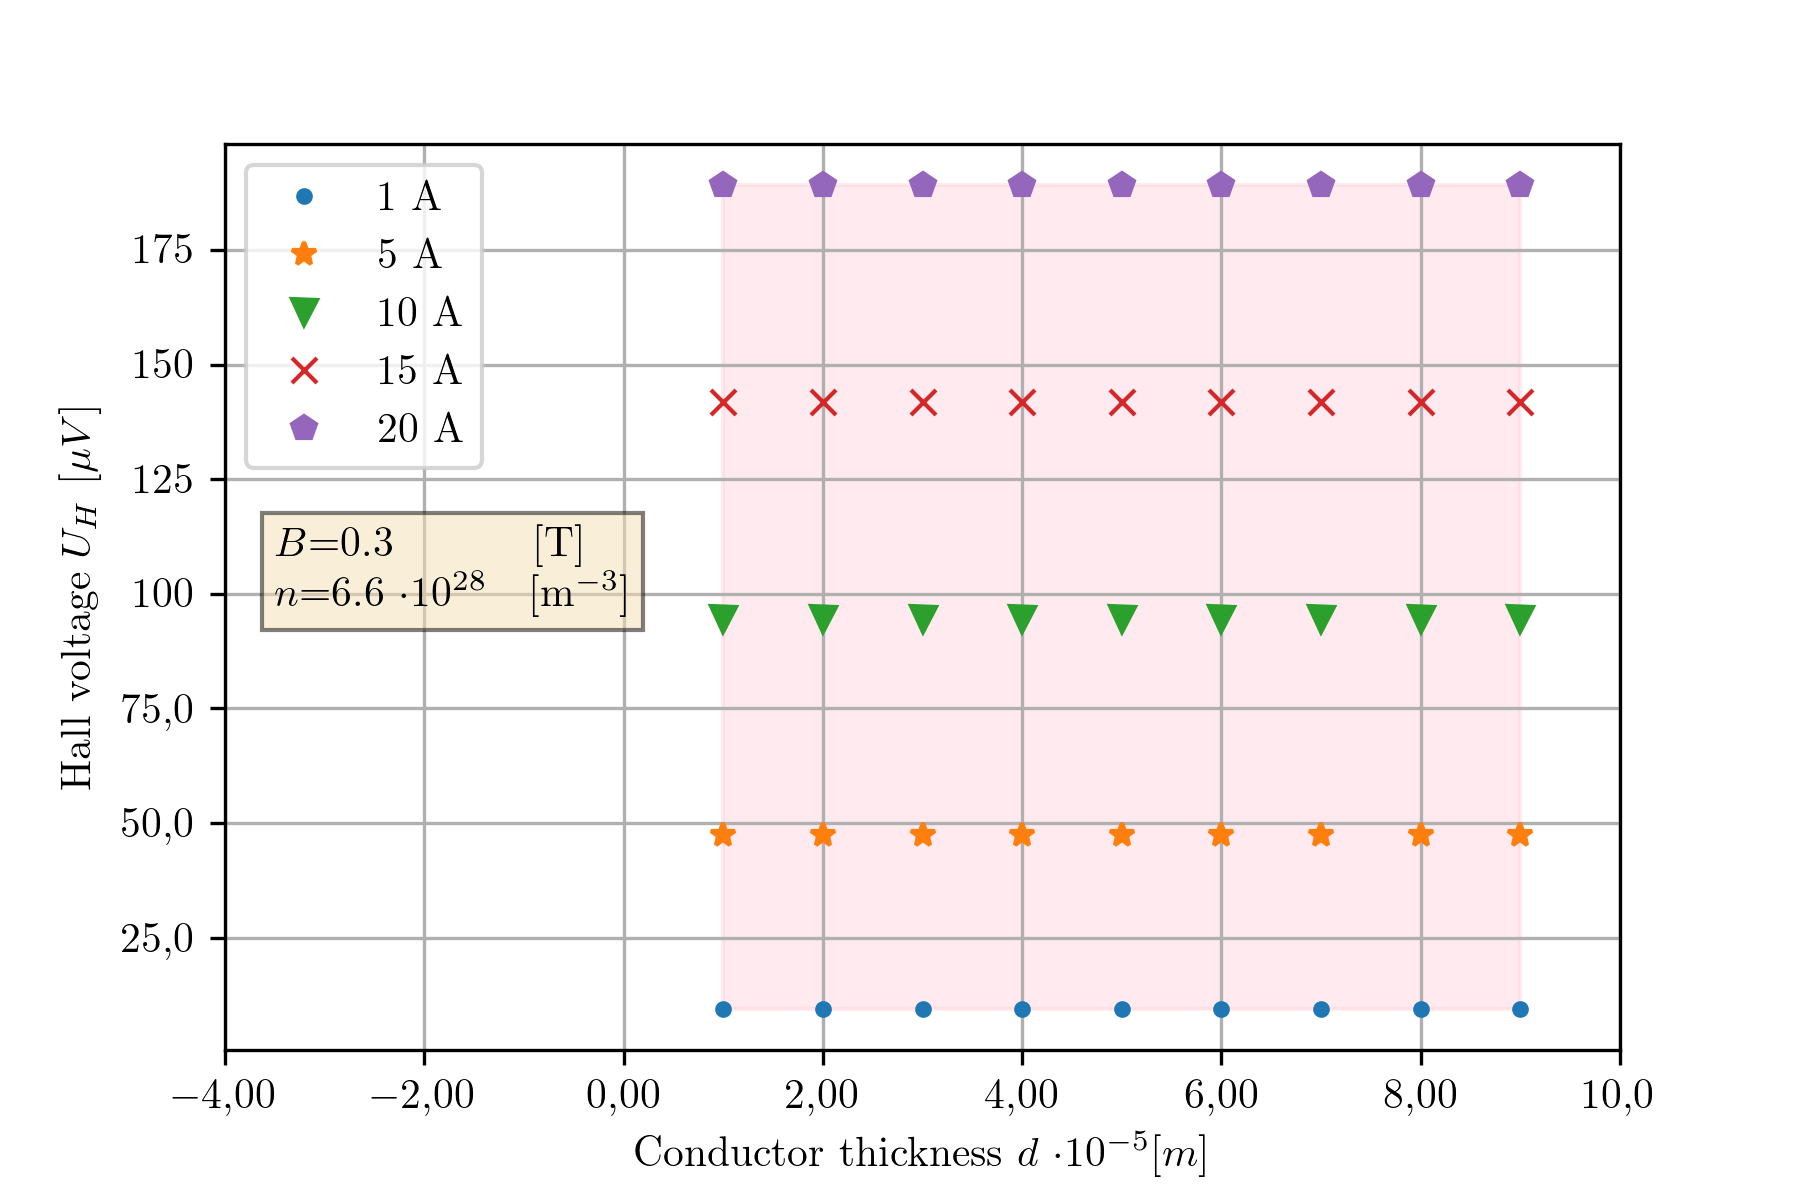
\includegraphics[scale=0.9]{figuren/simulatie/d.png} 
    \end{center}
    \caption{Simulation result of Formula \ref{eq:Hall Voltage2}.} \label{fig:sim_d}
    \end{figure}
    
    \begin{figure}[!htbp]
    \begin{center}
    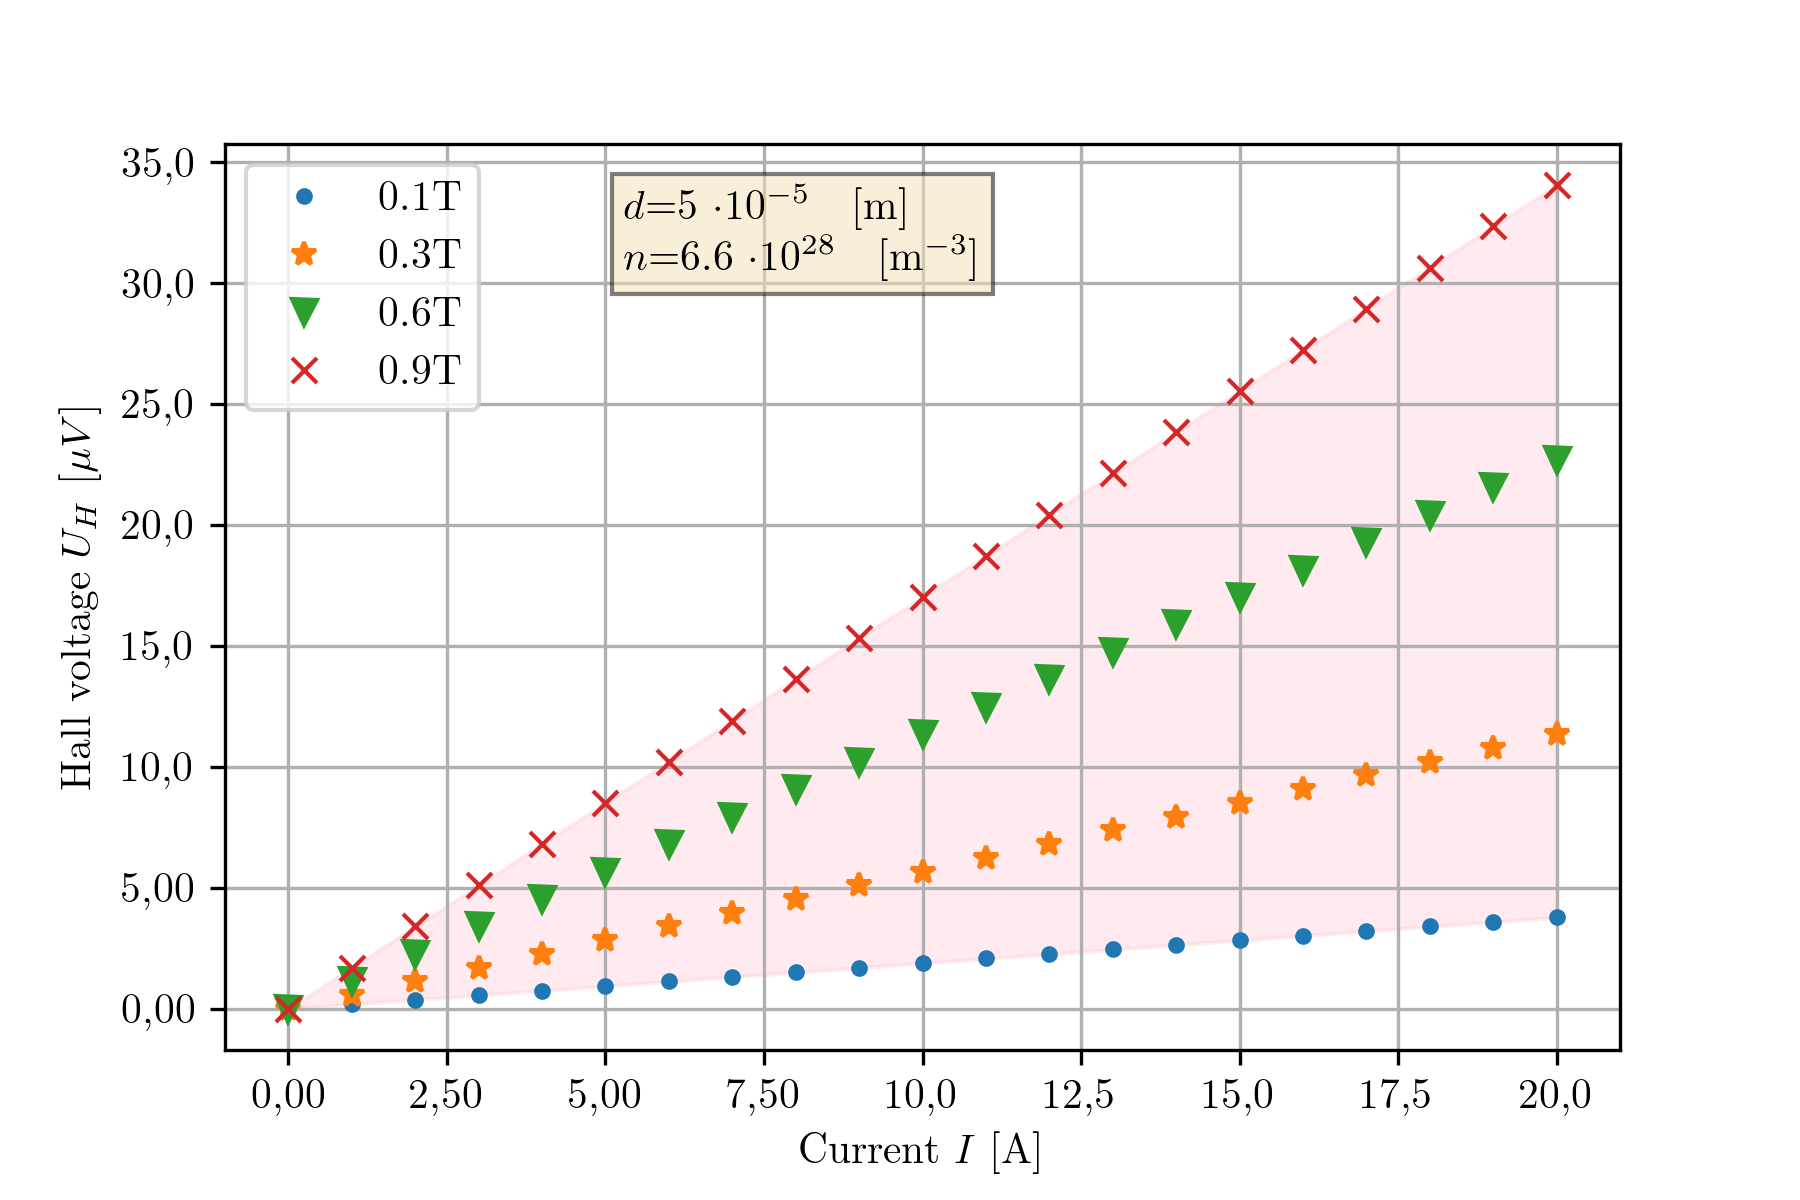
\includegraphics[scale=0.9]{figuren/simulatie/I.png}
    \end{center}
    \caption{Simulation result of Formula \ref{eq:Hall Voltage2}.}  \label{fig:sim_I}
    \end{figure}

    \begin{figure}[!htbp]
    \begin{center}
    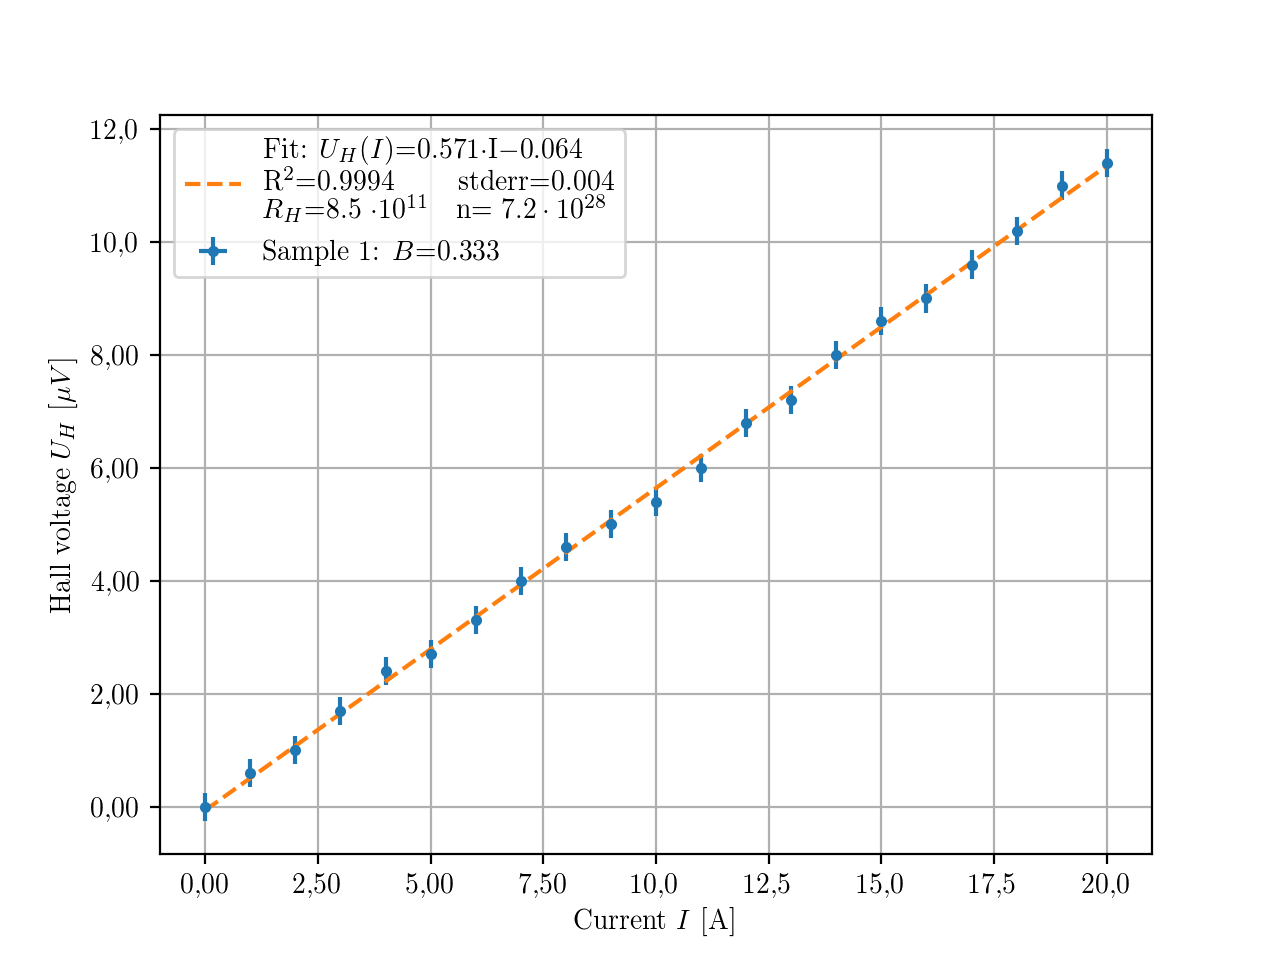
\includegraphics[scale=0.8]{figuren/resultaten/sample1.png}
    \end{center}
    \caption{Results sample 1 of the Hall voltage measurement with the Hall apparatus (silver).}\label{fig:silver1}
    \end{figure}
    

    \begin{figure}[!htbp]
    \begin{center}
    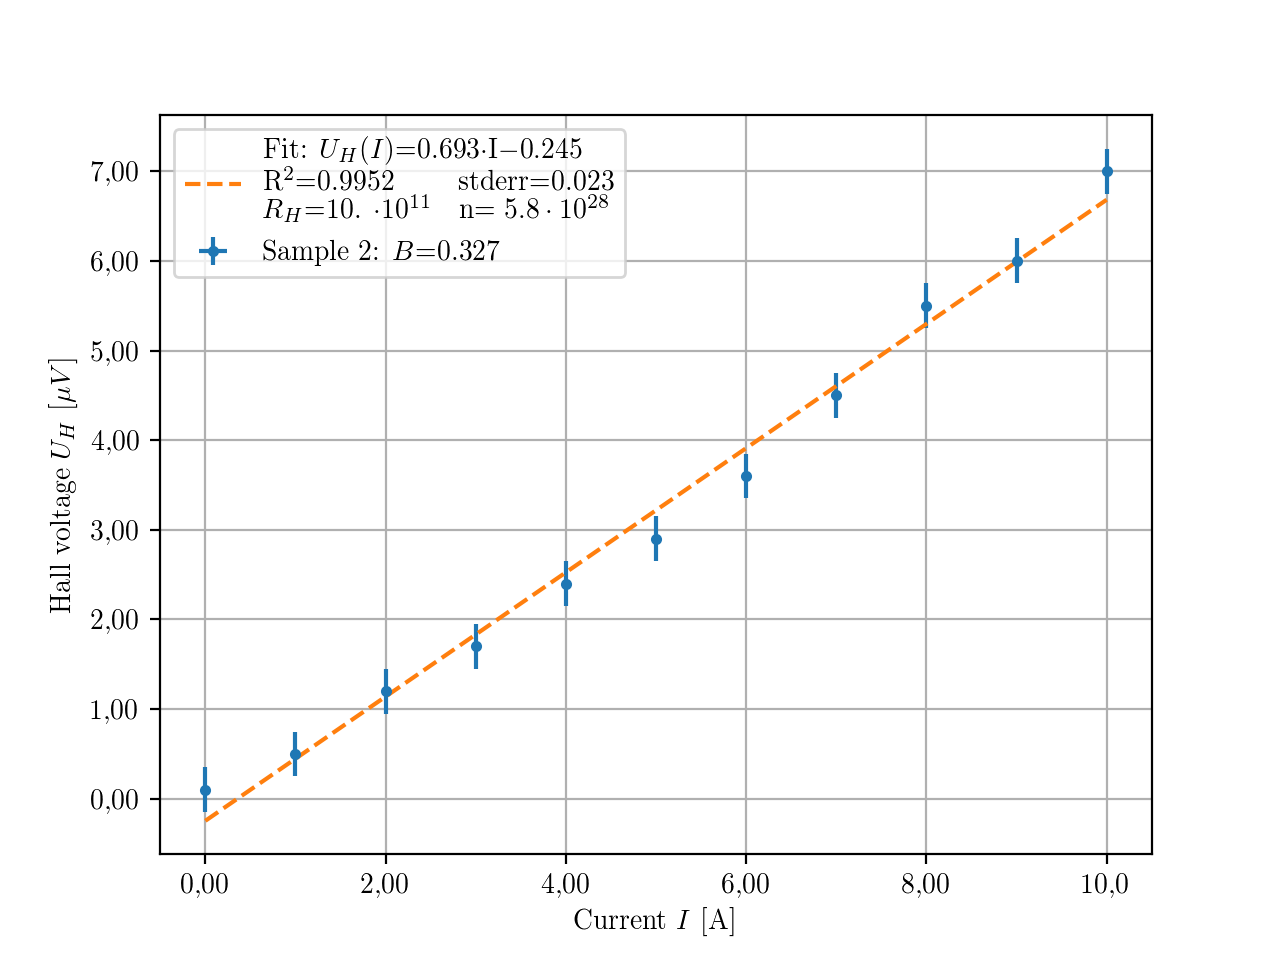
\includegraphics[scale=0.8]{figuren/resultaten/sample2.png}
    \end{center}
    \caption{Results sample 2 of the Hall voltage measurement with the Hall apparatus (silver).}\label{fig:silver2}
    \end{figure}
    
    \begin{figure}[!htbp]
    \begin{center}
    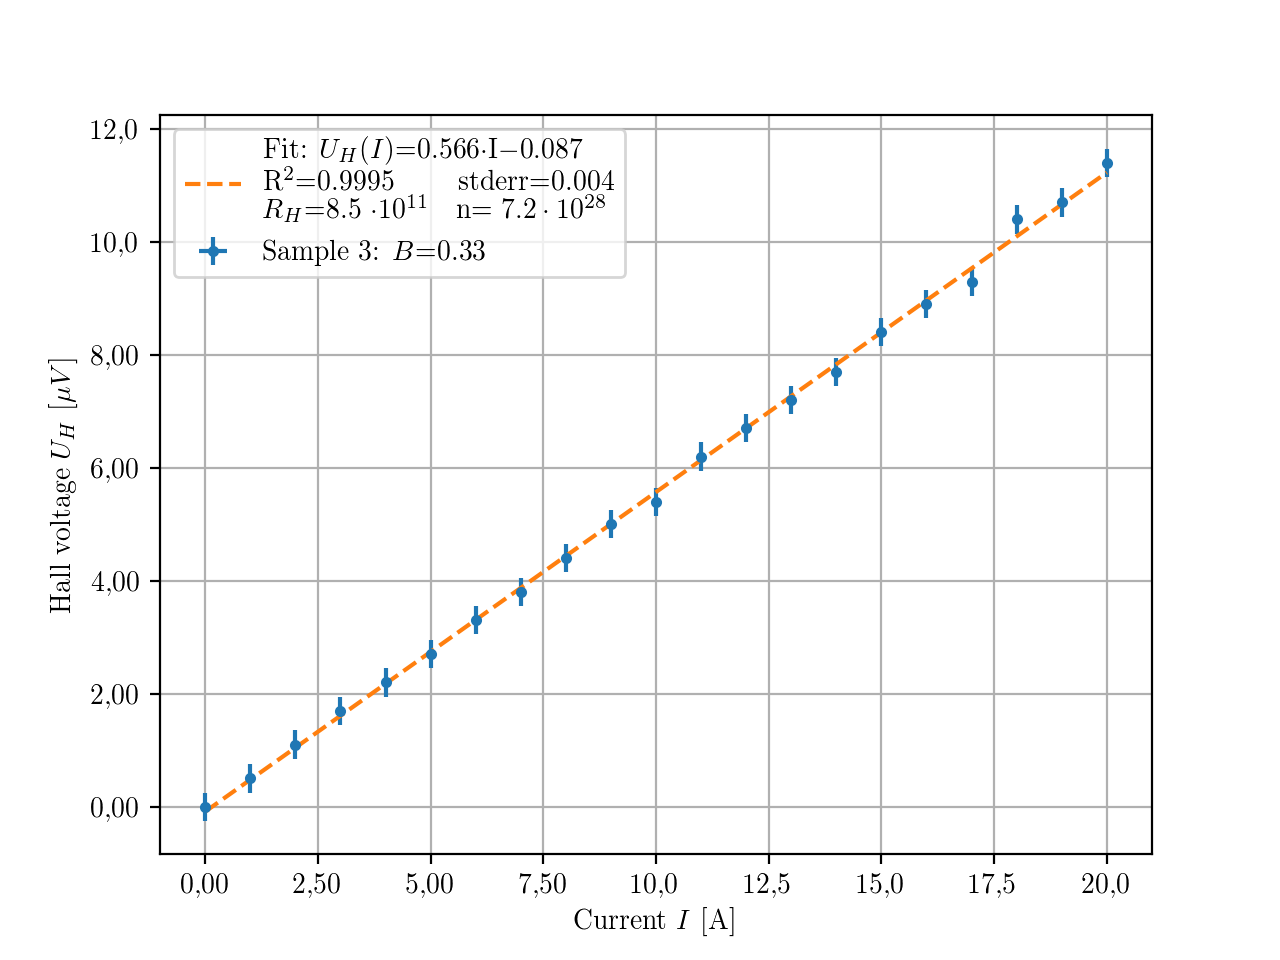
\includegraphics[scale=0.8]{figuren/resultaten/sample3.png}
    \end{center}
    \caption{Results sample 3 of the Hall voltage measurement with the Hall apparatus (silver).}\label{fig:silver3}
    \end{figure}
    
    \begin{figure}[!htbp]
    \begin{center}
    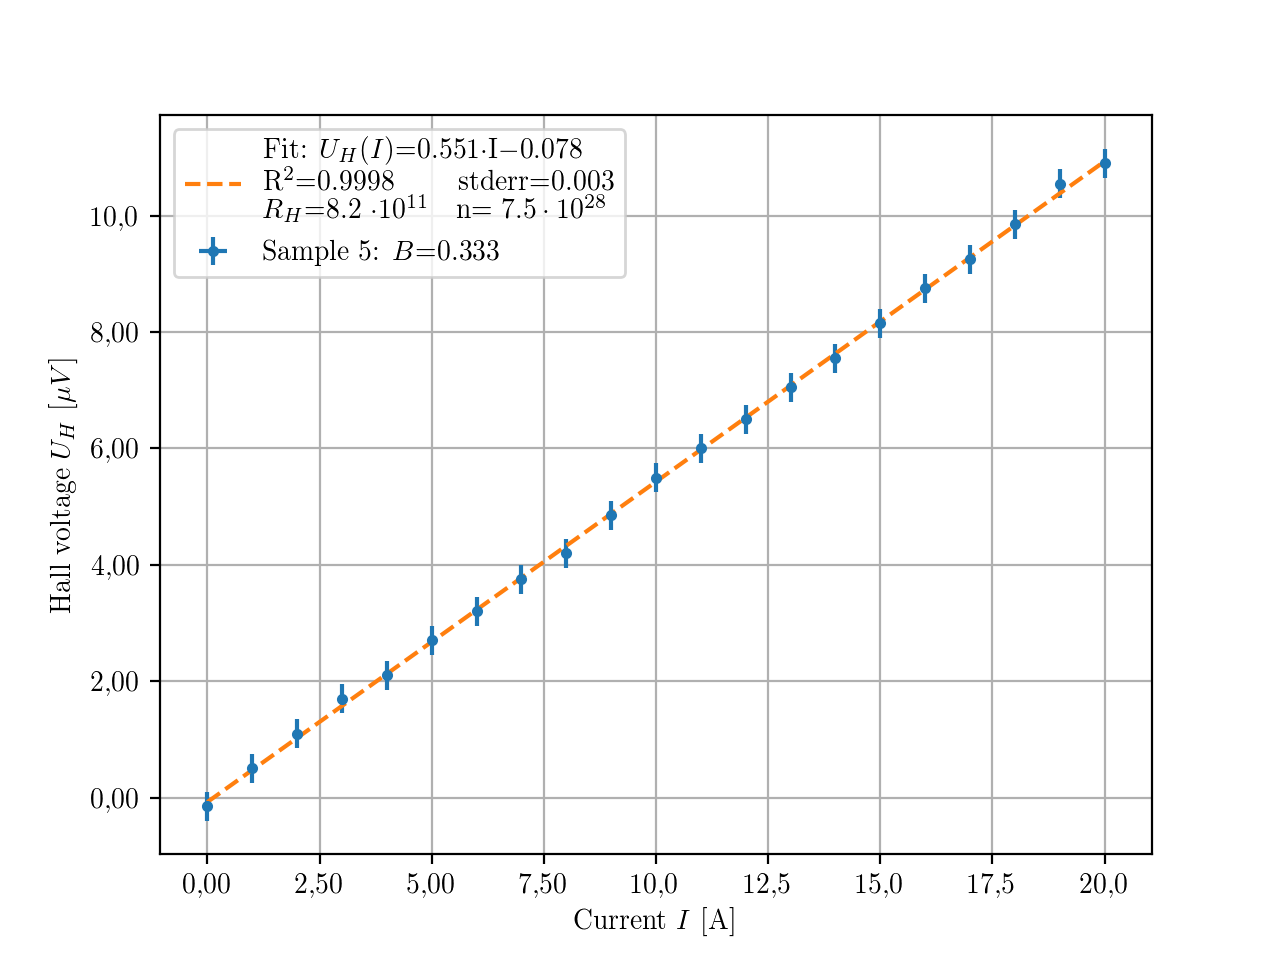
\includegraphics[scale=0.8]{figuren/resultaten/sample5.png}
    \end{center}
    \caption{Results sample 4 of the Hall voltage measurement with the Hall apparatus (silver).}\label{fig:silver4}
    \end{figure}
    
    \begin{figure}[!htbp]
    \begin{center}
    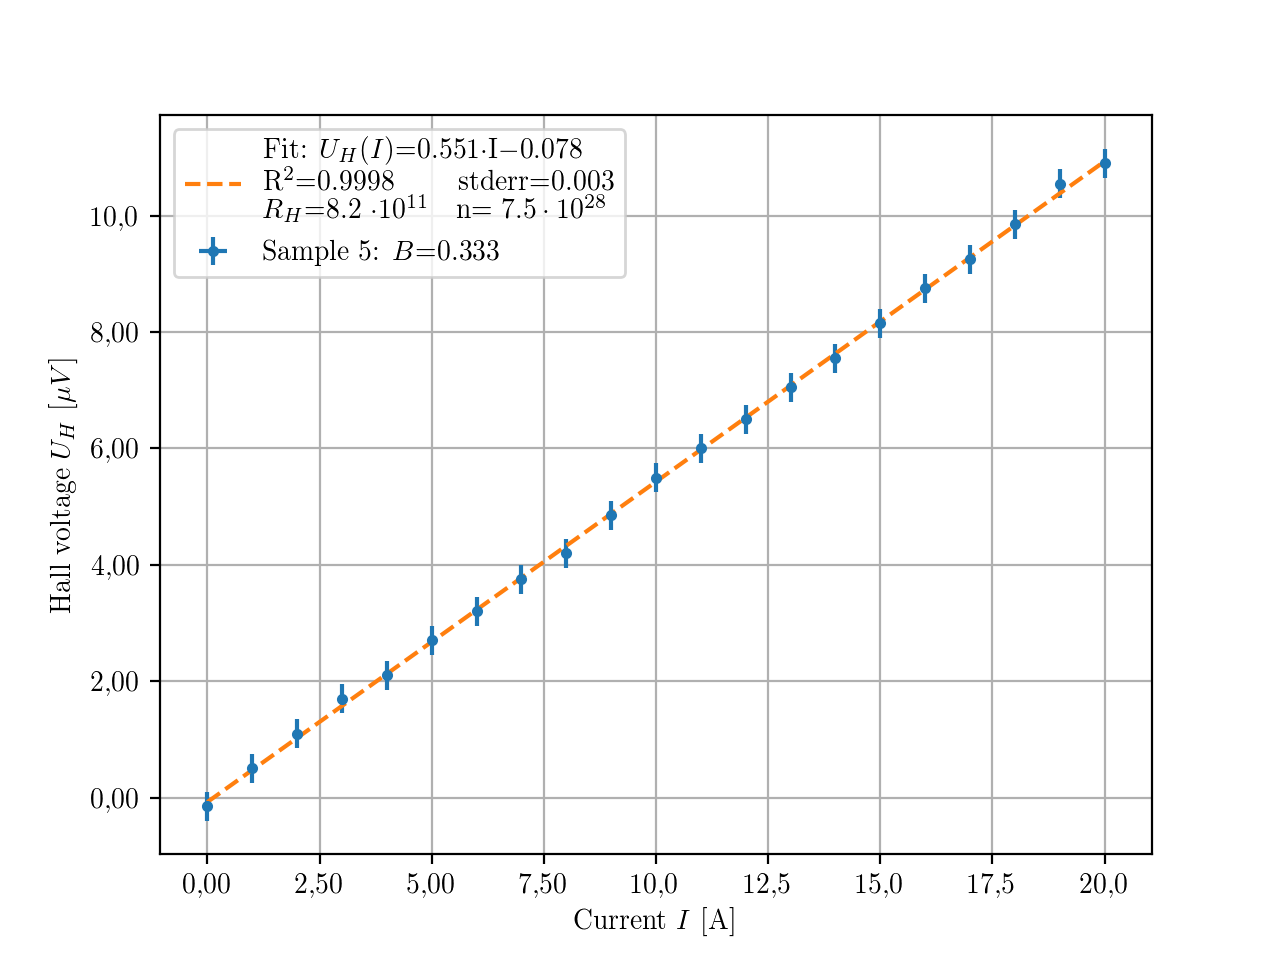
\includegraphics[scale=0.8]{figuren/resultaten/sample5.png}
    \end{center}
    \caption{Results sample 5 of the Hall voltage measurement with the Hall apparatus (silver).}\label{fig:silver5}
    \end{figure}
\lstset{ 
  backgroundcolor=\color{white},   % choose the background color; you must add \usepackage{color} or \usepackage{xcolor}; should come as last argument
  %basicstyle=\footnotesize,        % the size of the fonts that are used for the code
  %breakatwhitespace=false,         % sets if automatic breaks should only happen at whitespace
  breaklines=true,                 % sets automatic line breaking
  captionpos=b,                    % sets the caption-position to bottom
  %commentstyle=\color{red},    % comment style
  %deletekeywords={...},            % if you want to delete keywords from the given language
  %escapeinside={\%*}{*)},          % if you want to add LaTeX within your code
  %extendedchars=true,              % lets you use non-ASCII characters; for 8-bits encodings only, does %not work with UTF-8
  frame=leftline,	                   % adds a frame around the code
  keepspaces=true,                 % keeps spaces in text, useful for keeping indentation of code (possibly needs columns=flexible)
  %keywordstyle=\color{blue},       % keyword style
  language=Python,                 % the language of the code
  %morekeywords={*,...},            % if you want to add more keywords to the set
  numbers=left,                    % where to put the line-numbers; possible values are (none, left, right)
  %numbersep=5pt,                   % how far the line-numbers are from the code
  %numberstyle=\tiny\color{mygray}, % the style that is used for the line-numbers
  %rulecolor=\color{green},         % if not set, the frame-color may be changed on line-breaks within not-black text (e.g. comments (green here))
  stepnumber=2,                    % the step between two line-numbers. If it's 1, each line will be numbered
  %stringstyle=\color{mymauve},     % string literal style
  %tabsize=2,	                   % sets default tabsize to 2 spaces
  %title=\lstname                   % show the filename of files included with \lstinputlisting; also try caption instead of title
} %vereist voor python opmaak
\chapter{Python code}
\section{Dataverwerking Life Time Meting}
\label{Bijlage2DataverwerkingLifeTimeMeting}
\lstinputlisting{appendix/python/Life_time_verwerking.py}

\section{Dataverwerking Delta Time Meting}
\label{Bijlage2DataverwerkingLifeTimeMeting}
\lstinputlisting{appendix/python/Delta_time_verwerking.py}
\chapter{Required appendix}
    Gezien dit de bijlage is en het twee onderdelen bevat welke als vereiste moeten worden toegevoegd aan de bijlage word dit onderdeel in het Nederlands geschreven.
    
\section{Verantwoording}
In deze sectie word omschreven wat de individuele bijdrages zijn geweest van beide duo-leden.
    \subsection{Brian de Keijzer}
    ...
    \subsection{Julia Norbart}
    ...

\section{Zelfreflectie}
Deze sectie bevat de zelfreflectie van beide duo-leden.
    \subsection{Brian de Keijzer}
    ...
    \subsection{Julia Norbart}
    ...



\end{document}